\documentclass[12pt,halfline,a4paper,]{ouparticle}

% Packages I think are necessary for basic Rmarkdown functionality
\usepackage{hyperref}
\usepackage{graphicx}
\usepackage{listings}
\usepackage{color}
\usepackage{fancyvrb}
\usepackage{framed}

% For knitr::kable functionality
\usepackage{booktabs}
\usepackage{longtable}

%% To allow better options for figure placement
%\usepackage{float}

% Packages that are supposedly required by OUP sty file
\usepackage{amssymb, amsmath, geometry, amsfonts, verbatim, endnotes, setspace}

% For code highlighting I think
\DefineVerbatimEnvironment{Highlighting}{Verbatim}{commandchars=\\\{\}}
\definecolor{shadecolor}{RGB}{248,248,248}
\newenvironment{Shaded}{\begin{snugshade}}{\end{snugshade}}
\newcommand{\AlertTok}[1]{\textcolor[rgb]{0.94,0.16,0.16}{#1}}
\newcommand{\AnnotationTok}[1]{\textcolor[rgb]{0.56,0.35,0.01}{\textbf{\textit{#1}}}}
\newcommand{\AttributeTok}[1]{\textcolor[rgb]{0.77,0.63,0.00}{#1}}
\newcommand{\BaseNTok}[1]{\textcolor[rgb]{0.00,0.00,0.81}{#1}}
\newcommand{\BuiltInTok}[1]{#1}
\newcommand{\CharTok}[1]{\textcolor[rgb]{0.31,0.60,0.02}{#1}}
\newcommand{\CommentTok}[1]{\textcolor[rgb]{0.56,0.35,0.01}{\textit{#1}}}
\newcommand{\CommentVarTok}[1]{\textcolor[rgb]{0.56,0.35,0.01}{\textbf{\textit{#1}}}}
\newcommand{\ConstantTok}[1]{\textcolor[rgb]{0.00,0.00,0.00}{#1}}
\newcommand{\ControlFlowTok}[1]{\textcolor[rgb]{0.13,0.29,0.53}{\textbf{#1}}}
\newcommand{\DataTypeTok}[1]{\textcolor[rgb]{0.13,0.29,0.53}{#1}}
\newcommand{\DecValTok}[1]{\textcolor[rgb]{0.00,0.00,0.81}{#1}}
\newcommand{\DocumentationTok}[1]{\textcolor[rgb]{0.56,0.35,0.01}{\textbf{\textit{#1}}}}
\newcommand{\ErrorTok}[1]{\textcolor[rgb]{0.64,0.00,0.00}{\textbf{#1}}}
\newcommand{\ExtensionTok}[1]{#1}
\newcommand{\FloatTok}[1]{\textcolor[rgb]{0.00,0.00,0.81}{#1}}
\newcommand{\FunctionTok}[1]{\textcolor[rgb]{0.00,0.00,0.00}{#1}}
\newcommand{\ImportTok}[1]{#1}
\newcommand{\InformationTok}[1]{\textcolor[rgb]{0.56,0.35,0.01}{\textbf{\textit{#1}}}}
\newcommand{\KeywordTok}[1]{\textcolor[rgb]{0.13,0.29,0.53}{\textbf{#1}}}
\newcommand{\NormalTok}[1]{#1}
\newcommand{\OperatorTok}[1]{\textcolor[rgb]{0.81,0.36,0.00}{\textbf{#1}}}
\newcommand{\OtherTok}[1]{\textcolor[rgb]{0.56,0.35,0.01}{#1}}
\newcommand{\PreprocessorTok}[1]{\textcolor[rgb]{0.56,0.35,0.01}{\textit{#1}}}
\newcommand{\RegionMarkerTok}[1]{#1}
\newcommand{\SpecialCharTok}[1]{\textcolor[rgb]{0.00,0.00,0.00}{#1}}
\newcommand{\SpecialStringTok}[1]{\textcolor[rgb]{0.31,0.60,0.02}{#1}}
\newcommand{\StringTok}[1]{\textcolor[rgb]{0.31,0.60,0.02}{#1}}
\newcommand{\VariableTok}[1]{\textcolor[rgb]{0.00,0.00,0.00}{#1}}
\newcommand{\VerbatimStringTok}[1]{\textcolor[rgb]{0.31,0.60,0.02}{#1}}
\newcommand{\WarningTok}[1]{\textcolor[rgb]{0.56,0.35,0.01}{\textbf{\textit{#1}}}}

% For making Rmarkdown lists
\providecommand{\tightlist}{%
  \setlength{\itemsep}{0pt}\setlength{\parskip}{0pt}}

% Part for setting citation format package: natbib

% Part for setting citation format package: biblatex

% Part for indenting CSL refs
\newlength{\cslhangindent}
\setlength{\cslhangindent}{1.5em}
\newenvironment{cslreferences}%
  {\setlength{\parindent}{0pt}%
  \everypar{\setlength{\hangindent}{\cslhangindent}}\ignorespaces}%
  {\par}

% Pandoc header
\usepackage[nomarkers,tablesfirst]{endfloat}
\usepackage{lineno}
\linenumbers

\begin{document}

\title{Template for Oxford University Press papers}

\author{%
\name{Qiushi Yan}\address{Some Institute of Technology}\email{\href{mailto:qiushi.yann@gmail.com}{qiushi.yann@gmail.com}}
}

\abstract{This is the abstract.

It consists of two paragraphs.}

\date{\today}

\keywords{key; dictionary; word}

\maketitle



\hypertarget{introduction}{%
\section{Introduction}\label{introduction}}

cross reference using different syntax, see source

no bookdown latex environment

This template is based on the generic OUP template available \href{https://academic.oup.com/icesjms/pages/General_Instructions}{here}. The original OUP sample tex document, providing more details on prefered formatting for LaTeX documents, is included with the template in the file \texttt{ouparticle\_sample.tex}.

Here are two sample references: Feynman and Vernon Jr. (1963; Dirac 1953). Bibliography will appear at the end of the document.

\href{qiushi.rbind.io}{links}

\hypertarget{chapter-2}{%
\section{Chapter 2}\label{chapter-2}}

cross referencing figures \ref{fig:diamond}

\begin{figure}[p]
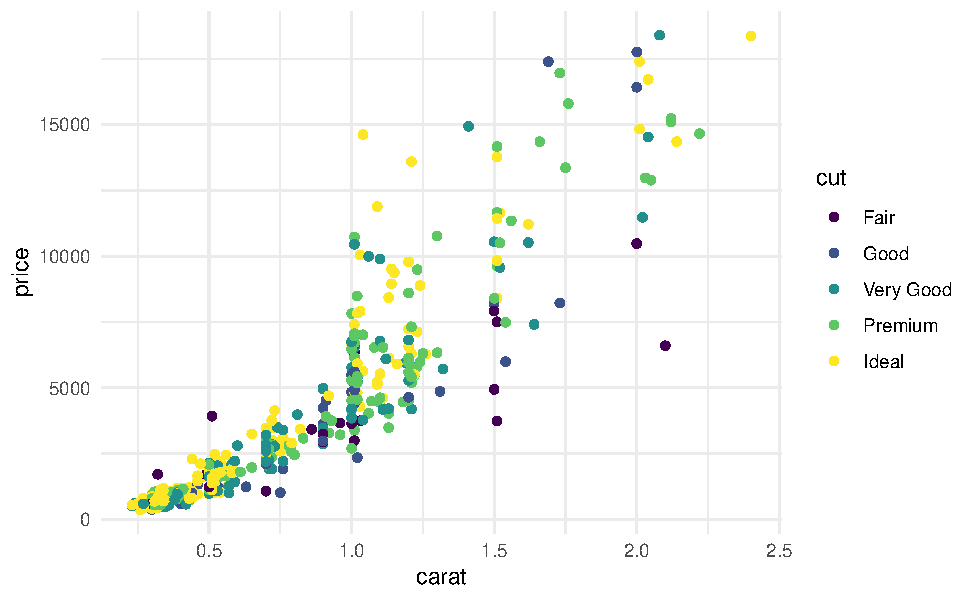
\includegraphics[width=1\linewidth]{oxford-press_files/figure-latex/diamond-1} \caption{this is a figure}\label{fig:diamond}
\end{figure}

cross referencing tables \ref{tab:iris}

\begin{table}

\caption{\label{tab:iris}my table}
\centering
\begin{tabular}[t]{r|r|r|r|l}
\hline
Sepal.Length & Sepal.Width & Petal.Length & Petal.Width & Species\\
\hline
5.1 & 3.5 & 1.4 & 0.2 & setosa\\
\hline
4.9 & 3.0 & 1.4 & 0.2 & setosa\\
\hline
4.7 & 3.2 & 1.3 & 0.2 & setosa\\
\hline
4.6 & 3.1 & 1.5 & 0.2 & setosa\\
\hline
5.0 & 3.6 & 1.4 & 0.2 & setosa\\
\hline
5.4 & 3.9 & 1.7 & 0.4 & setosa\\
\hline
\end{tabular}
\end{table}

\hypertarget{materials-and-methods}{%
\section{Materials and methods}\label{materials-and-methods}}

An equation with a label for cross-referencing:

\begin{equation}\label{eq:eq1}
\int^{r_2}_0 F(r,\varphi){\rm d}r\,{\rm d}\varphi = [\sigma r_2/(2\mu_0)]
\int^{\infty}_0\exp(-\lambda|z_j-z_i|)\lambda^{-1}J_1 (\lambda r_2)J_0
(\lambda r_i\,\lambda {\rm d}\lambda)
\end{equation}

This equation can be referenced as follows: Eq. \ref{eq:eq1}

\hypertarget{a-subsection}{%
\subsection{A subsection}\label{a-subsection}}

A numbered list:

\begin{enumerate}
\def\labelenumi{\arabic{enumi})}
\tightlist
\item
  First point
\item
  Second point

  \begin{itemize}
  \tightlist
  \item
    Subpoint
  \end{itemize}
\end{enumerate}

A bullet list:

\begin{itemize}
\tightlist
\item
  First point
\item
  Second point
\end{itemize}

\hypertarget{results}{%
\section{Results}\label{results}}

\hypertarget{generate-a-figure.}{%
\subsection{Generate a figure.}\label{generate-a-figure.}}

\begin{Shaded}
\begin{Highlighting}[]
\KeywordTok{plot}\NormalTok{(}\DecValTok{1}\OperatorTok{:}\DecValTok{10}\NormalTok{,}\DataTypeTok{main=}\StringTok{"Some data"}\NormalTok{,}\DataTypeTok{xlab=}\StringTok{"Distance (cm)"}\NormalTok{,}\DataTypeTok{ylab=}\StringTok{"Time (hours)"}\NormalTok{)}
\end{Highlighting}
\end{Shaded}

\begin{figure}[p]
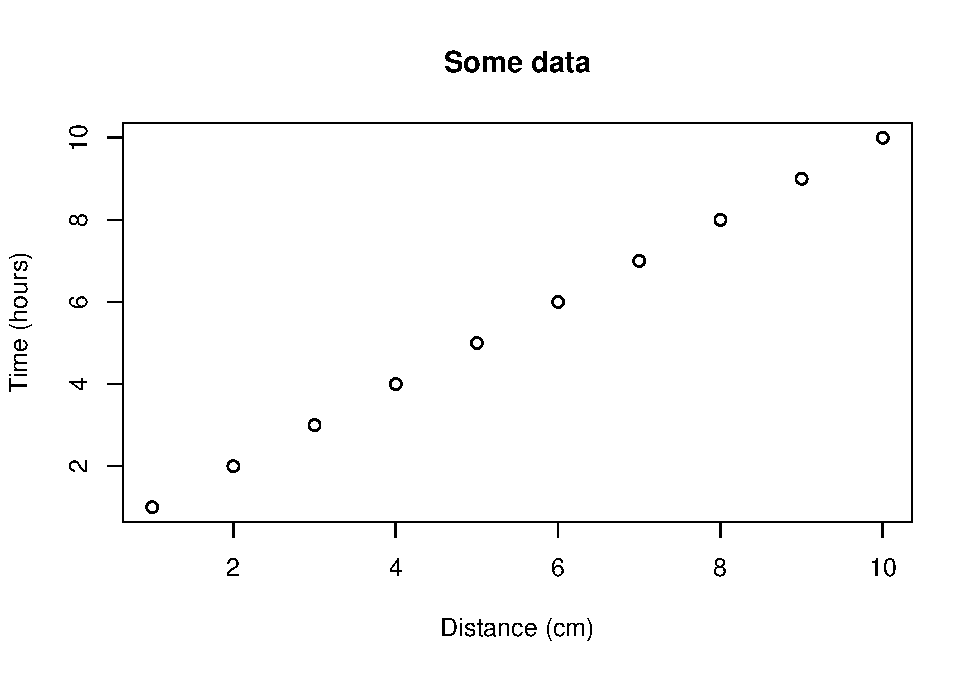
\includegraphics[width=1\linewidth]{oxford-press_files/figure-latex/fig1-1} \caption{This is the first figure.}\label{fig:fig1}
\end{figure}

You can reference this figure as follows: Fig. \ref{fig:fig1}.

\begin{Shaded}
\begin{Highlighting}[]
\KeywordTok{plot}\NormalTok{(}\DecValTok{1}\OperatorTok{:}\DecValTok{5}\NormalTok{,}\DataTypeTok{pch=}\DecValTok{19}\NormalTok{,}\DataTypeTok{main=}\StringTok{"Some data"}\NormalTok{,}\DataTypeTok{xlab=}\StringTok{"Distance (cm)"}\NormalTok{,}\DataTypeTok{ylab=}\StringTok{"Time (hours)"}\NormalTok{)}
\end{Highlighting}
\end{Shaded}

\begin{figure}[p]
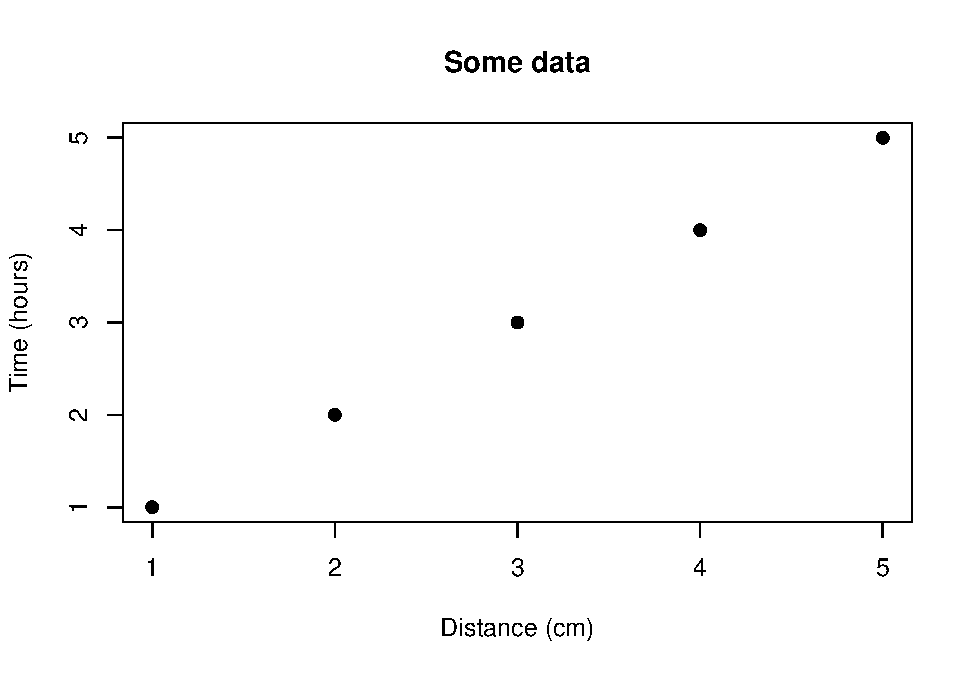
\includegraphics[width=1\linewidth]{oxford-press_files/figure-latex/fig2-1} \caption{This is the second figure.}\label{fig:fig2}
\end{figure}

Reference to second figure: Fig. \ref{fig:fig2}

\hypertarget{generate-a-table-using-xtable}{%
\subsection{\texorpdfstring{Generate a table using \texttt{xtable}}{Generate a table using xtable}}\label{generate-a-table-using-xtable}}

\begin{Shaded}
\begin{Highlighting}[]
\NormalTok{df =}\StringTok{ }\KeywordTok{data.frame}\NormalTok{(}\DataTypeTok{ID=}\DecValTok{1}\OperatorTok{:}\DecValTok{3}\NormalTok{,}\DataTypeTok{code=}\NormalTok{letters[}\DecValTok{1}\OperatorTok{:}\DecValTok{3}\NormalTok{])}

\CommentTok{\# Creates tables that follow OUP guidelines using xtable}
\KeywordTok{library}\NormalTok{(xtable) }
\KeywordTok{print}\NormalTok{(}\KeywordTok{xtable}\NormalTok{(df,}\DataTypeTok{caption=}\StringTok{"This is the table caption"}\NormalTok{,}\DataTypeTok{label=}\StringTok{"tab:tab1"}\NormalTok{),}
      \DataTypeTok{comment=}\OtherTok{FALSE}\NormalTok{)}
\end{Highlighting}
\end{Shaded}

\begin{table}[ht]
\centering
\begin{tabular}{rrl}
  \hline
 & ID & code \\ 
  \hline
1 &   1 & a \\ 
  2 &   2 & b \\ 
  3 &   3 & c \\ 
   \hline
\end{tabular}
\caption{This is the table caption} 
\label{tab:tab1}
\end{table}

You can reference this table as follows: Table \ref{tab:tab1}.

\hypertarget{generate-a-table-using-kable}{%
\subsection{\texorpdfstring{Generate a table using \texttt{kable}}{Generate a table using kable}}\label{generate-a-table-using-kable}}

\begin{Shaded}
\begin{Highlighting}[]
\NormalTok{df =}\StringTok{ }\KeywordTok{data.frame}\NormalTok{(}\DataTypeTok{ID=}\DecValTok{1}\OperatorTok{:}\DecValTok{3}\NormalTok{,}\DataTypeTok{code=}\NormalTok{letters[}\DecValTok{1}\OperatorTok{:}\DecValTok{3}\NormalTok{])}

\CommentTok{\# kable can alse be used for creating tables}
\NormalTok{knitr}\OperatorTok{::}\KeywordTok{kable}\NormalTok{(df,}\DataTypeTok{caption=}\StringTok{"This is the table caption"}\NormalTok{,}\DataTypeTok{format=}\StringTok{"latex"}\NormalTok{,}
             \DataTypeTok{booktabs=}\OtherTok{TRUE}\NormalTok{,}\DataTypeTok{label=}\StringTok{"tab2"}\NormalTok{)}
\end{Highlighting}
\end{Shaded}

\begin{table}

\caption{\label{tab:tab2}This is the table caption}
\centering
\begin{tabular}[t]{rl}
\toprule
ID & code\\
\midrule
1 & a\\
2 & b\\
3 & c\\
\bottomrule
\end{tabular}
\end{table}

You can reference this table as follows: Table \ref{tab:tab2}.

\hypertarget{discussion}{%
\section{Discussion}\label{discussion}}

You can cross-reference sections and subsections as follows: Section \ref{materials-and-methods} and Section \ref{a-subsection}.

\textbf{\emph{Note:}} the last section in the document will be used as the section title for the bibliography.

\hypertarget{references}{%
\section*{References}\label{references}}
\addcontentsline{toc}{section}{References}

\hypertarget{refs}{}
\begin{cslreferences}
\leavevmode\hypertarget{ref-Dirac1953888}{}%
Dirac, P. A. M. 1953. ``The Lorentz Transformation and Absolute Time.'' \emph{Physica} 19 (1-\/--12): 888--96. \url{https://doi.org/10.1016/S0031-8914(53)80099-6}.

\leavevmode\hypertarget{ref-Feynman1963118}{}%
Feynman, R. P, and F. L Vernon Jr. 1963. ``The Theory of a General Quantum System Interacting with a Linear Dissipative System.'' \emph{Annals of Physics} 24: 118--73. \url{https://doi.org/10.1016/0003-4916(63)90068-X}.
\end{cslreferences}


\begin{notes}[Acknowledgements]
This is an acknowledgement.

It consists of two paragraphs.
\end{notes}




\end{document}
